\documentclass[11pt]{article}

\setlength\parindent{0pt}
\usepackage{graphicx}
\usepackage{hyperref}
\righthyphenmin = 62

\title{IT3105 Artificial Intelligence Programming \\ Module 1 - A* on Navigation Tasks}
\author{Johannes Moskvil}

\begin{document}
\maketitle

\section*{Central aspects of A* and the agenda loop}
A* is a local search algorithm similar to DFS and BFS searches, but differs from the others by using a heuristic in guiding the search toward the solution. This report describes the central aspects of my A* implementation for module 1.

\vspace{5mm}

The agenda is the main loop in A*. At each loop it pops a node from the open list until it either runs out of nodes or finds a solution. Currently there is no depth-limit to the search. \textit{Figure 1} shows the Python code for the implemented agenda loop. This is the general loop for many A* problems. In order to tailor the implementation to new problems one would simply need to write new methods for generating new successor states\footnote{Here a state corresponds to a node. The term Node and State will be used interchangeably in this report}, \textbf{GetNearbyNodes(Node)}, and \textbf{UpdateNodeCosts(Node, Node)} whose responsibility is to update the \textbf{g}, \textbf{h} and \textbf{f} values as well as the \textbf{parent} property for each node. 
This implementation also accounts for the possibility that one may want to find solutions for 'terrain-mazes', therefore the walls in this navigation-problem-instance are not modelled as 'not-passable', but rather have a large movement-cost associated with them. For this problem the agenda also contains a conditional check for skipping nodes whose movement-cost is greater than one, to reduce the number of nodes explored to reach the goal state. This implementation ensures that the agenda acts as a reusable core where other problem-specific details are implemented and taken care of in its template methods.

\begin{figure}[h]
\centerline{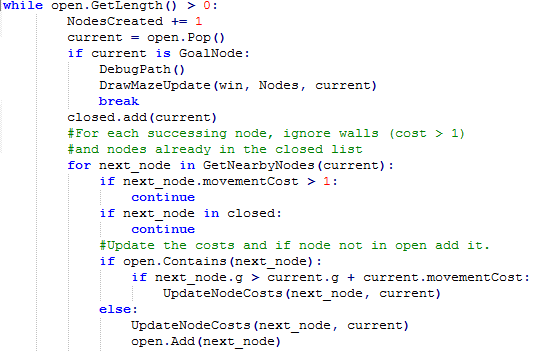
\includegraphics[scale=0.9]{Agenda_loop.png}}
\caption{Python code for the agenda loop}
\end{figure}

\vspace{5mm}

The heuristic function is what makes best-first searches different from BFS and DFS and guides the search toward a solution. For a navigation problem there are generally two options available: \textbf{Manhattan distance}, or \textbf{Euclidean distance}, see \textit{Figure 2}. 

\begin{figure}[h]
\centerline{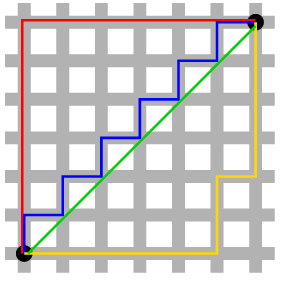
\includegraphics[scale=0.4]{Manhattan_distance_figure.png}}
\caption{Examples of Manhattan distances (red, blue and yellow) and Euclidean distances(green)}
\end{figure}


Since my implementation does not support diagonal moves, I chose the Manhattan distance as the heuristic. The Manhattan distance heuristic will give a very accurate estimate of the path towards the goal. If there is a clear path to the goal (no blocking wall) it gives a perfectly accurate estimate.

\begin{figure}[h]
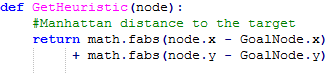
\includegraphics[scale=1.0]{heuristic_function.png}
\caption{The Manhattan distance used as heuristic}
\end{figure}


The A* algorithm takes one node at a time for the open list and expands it. In order to expand it, it needs a way to generate a list of next states. The agenda has a method called \textbf{GetNearbyNodes(Node)} which returns a list of neighboring nodes in the north,east,south and west direction, if they exist. See \textit{figure 4}. Even walls are returned by this function as the concept 'wall' is just a node with a very high movement cost. For these navigation problems generating the next states are quite trivial, but for other more advanced problem they may not be. But again, this would just require another implementation of \textbf{GetNearbyNodes(Node)}, but no changes to the agenda.


\begin{figure}[h]
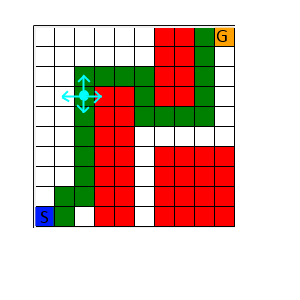
\includegraphics[scale=1.0]{Generate_Successor_States.png}
\caption{Successor states generated when expanding node(2,6)}
\end{figure}

\section*{REFERENCES}
- Manhattan Distance. Available from: \url{https://commons.wikimedia.org/wiki/File:Manhattan_distance.svg} [31 August 2015]
\end{document}